\documentclass{scrartcl}
\usepackage{graphicx}
\usepackage{float}
\usepackage[spanish]{babel}
\usepackage{hyperref} 
\graphicspath{ {img/} }
\setlength{\parskip}{\baselineskip}

\title{Tu Primera App para Android}
\subtitle{\large PAMN - Programación de Aplicaciónes Moviles Nativas}
\author{Chamil José Cruz Razeq}

\begin{document}
    \maketitle
    \thispagestyle{empty}
    \newpage

    \section{Introducción}
        Todas las tareas propuestas se encuentran disponibles en el siguiente
         repositorio de \href{https://github.com/chamilstudy/ulpgc_pamn_codeblocs1}{CodeBlocs1} y \href{https://github.com/chamilstudy/ulpgc_pamn_codeblocs1.2}{CodeBlocs1.2}.

    \section{Codeblocs 1: HappyBirthday}
        Aunque bastante guiado, este primer ejercicio plantea el workflow a seguir en el desarrollo
        de aplicaciones utilizando AndroidStudio, Kotlin y Compose. Presenta de manera efectiva como
        desarrollar el front end de la aplicación.
         \begin{figure}
            \centerline{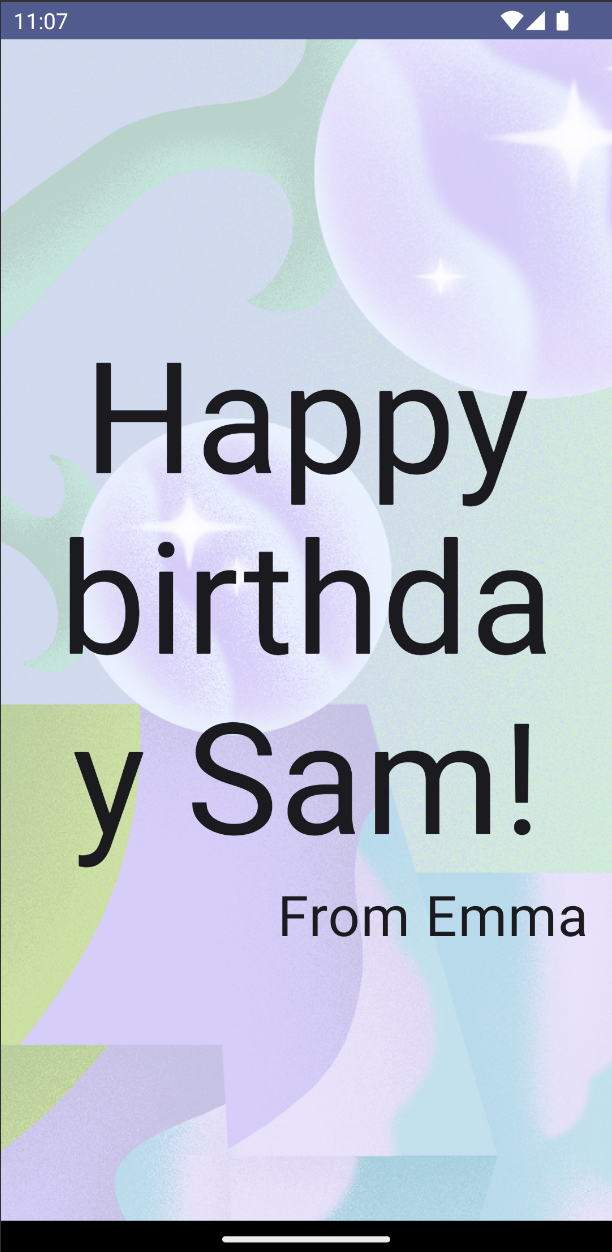
\includegraphics[scale=0.4]{birthday}}
            \caption{UI App codeblocs 1}
            \label{fig:birthday}
         \end{figure}
    \section{Codeblocs 1.2: Presentación}
        Este ejercicio, más avanzado, plantea la repetición de los pasos seguidos en el apartado anterior,
        pero ofreciendo una capa mas de dificultad, promoviendo que el desarrollador no solo tenga que revisar
        la documentación, sino utilizar nuevos elementos no planteados en el ejercicio anterior.
         \begin{figure}
            \centerline{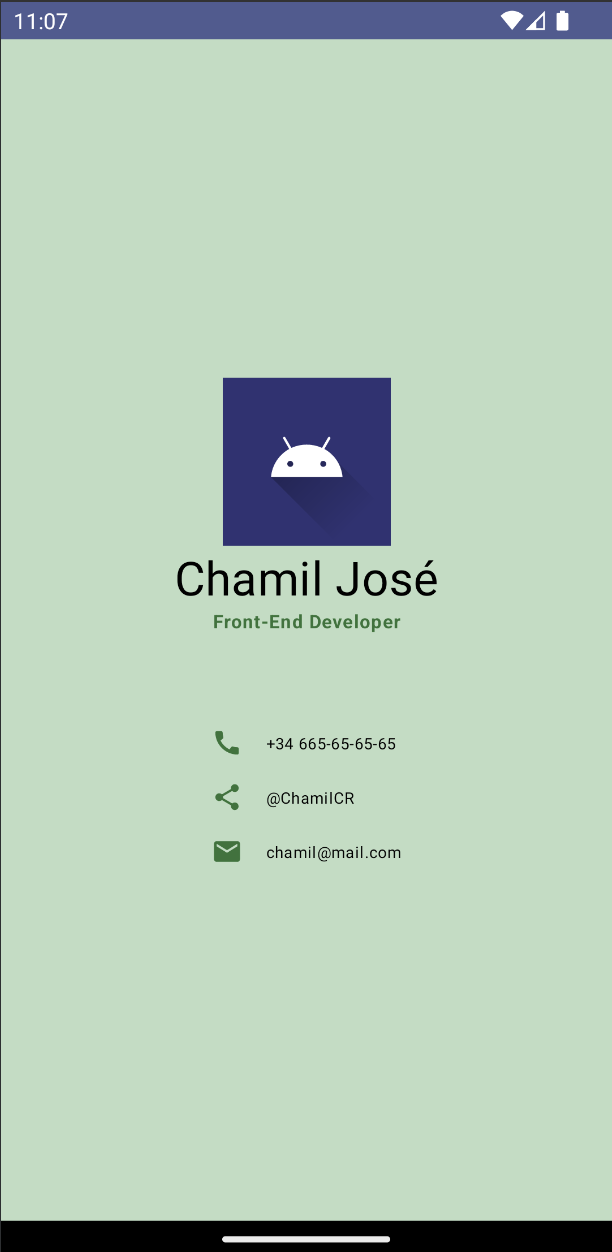
\includegraphics[scale=0.4]{presentacion}}
            \caption{UI App codeblocs 1.2}
            \label{fig:presentacion}
         \end{figure}
    
    \section{Conclusión}
         Como primer acercamiento al desarrollo de aplicaciones nativas, los codeblocs realizados presentan desarrollador
         manera ordenada un workflow, un nuevo lenguaje de programación y las peculiaridades del entorno.

\end{document}
